\documentclass{beamer}


\usepackage[francais]{babel}
\usepackage[T1]{fontenc}
\usepackage[utf8]{inputenc}


\usetheme{Warsaw}


\begin{document}


    \title {\textbf {Projet Hordes}}
    \author{Eric Tan - Younès Touffahi - Benjamin Rondeau}
    % \author{\href{mailto: eric.tan.etu@univ-lemans.fr} {younes.touffahi.etu@univ-lemans.fr} {benjamin.rondeau.etu@univ-lemans.fr}}
    \date{\today}
    \maketitle
    
    
    \begin{frame}
        \frametitle{Principe du jeu}
        \section{Principe du jeu}
        Hordes : jeu de survie, en ligne
        \\ Se joue quotidiennement sur de petites durées (10 minutes)
    \end{frame}
  
    
    \begin{frame}
        \frametitle{Conception}
        \section{Conception}
        Conception du jeu
        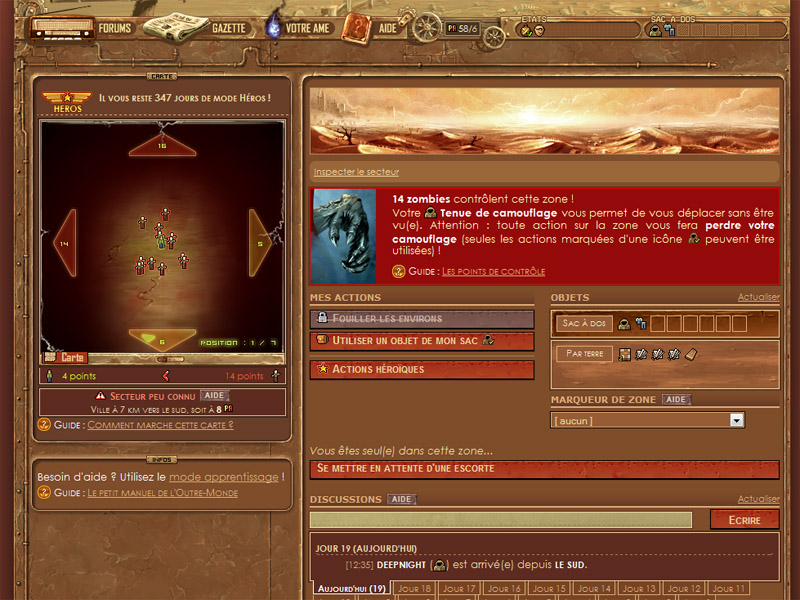
\includegraphics[width=\textwidth] {hordes.jpg}
    \end{frame}
    
    
    \begin{frame}
        \frametitle{Production}
        \framesubtitle{Boucle de jeu}
        \section{Production}
        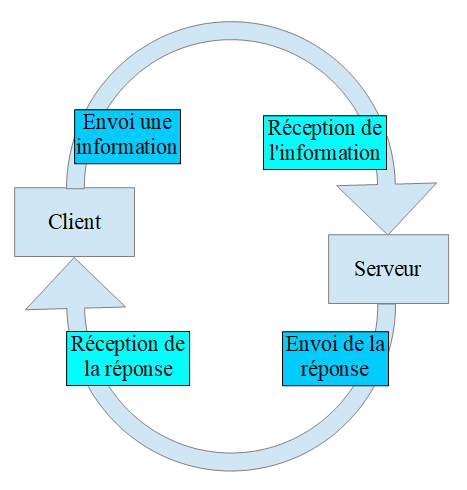
\includegraphics[width=5cm] {socket.PNG}
    \end{frame}
    
    
    \begin{frame}
        \frametitle{Production}
        \framesubtitle{Objets et Bâtiments}
        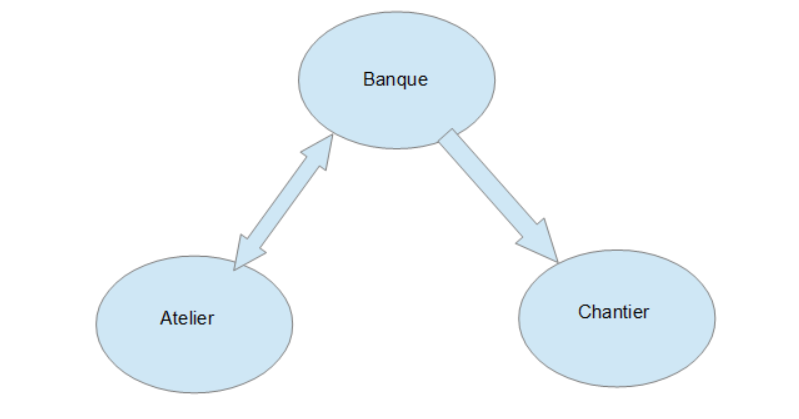
\includegraphics[width=\textwidth] {objet.PNG}
    \end{frame}
    
    
    \begin{frame}
        \frametitle{Production}
        \framesubtitle{Carte}
        La réalisation de la carte
        \\ et les mécaniques à l'extérieur de la ville
    \end{frame}
    
    
    \begin{frame}
        \frametitle{Production}
        \framesubtitle{Interface graphique}
        Réalisation d'une interface graphique
    \end{frame}
    
    
    \begin{frame}
        \frametitle{Résultat}
        \section{Résultat}
        Ce qu'on a réussi
        \\ ce qui n'a pas été achevé
    \end{frame}
    
    
    \begin{frame}
        \frametitle{Conclusion}
        \section{Conclusion}
        À retenir
    \end{frame}
    

\end{document}